\documentclass[11pt]{article}
\usepackage[textwidth=18.0cm, textheight=23.0cm, top=2.0cm]{geometry}
\usepackage{pst-all}
\usepackage{amssymb}
\usepackage{tikz}
\usepackage{underscore}\begin{document}
\pagestyle{empty}


ClassName: \underline{\textbf{Class_08.2bp-19}}
\par
BinSize: \underline{\textbf{100 × 100}}
\par
ReduceSize: \underline{\textbf{100 × 100}}
\par
TypeNum: \underline{\textbf{40}}
\par
Num: \underline{\textbf{40}}
\par
OutS: \underline{\textbf{130000}}
\par
InS: \underline{\textbf{105358}}
\par
Rate: \underline{\textbf{0.810}}
\par
UB: \underline{\textbf{13}}
\par
LB0: \underline{\textbf{13}}
\par
LB: \underline{\textbf{13}}
\par
LBWithCut: \underline{\textbf{13}}
\par
NodeCut: \underline{\textbf{0}}
\par
ExtendedNodeCnt: \underline{\textbf{1}}
\par
GenNodeCnt: \underline{\textbf{1}}
\par
PrimalNode: \underline{\textbf{0}}
\par
ColumnCount: \underline{\textbf{13}}
\par
TotalCutCount: \underline{\textbf{0}}
\par
RootCutCount: \underline{\textbf{0}}
\par
LPSolverCnt: \underline{\textbf{1}}
\par
PricingSolverCnt: \underline{\textbf{0}}
\par
BranchAndBoundNum: \underline{\textbf{1}}
\par
isOpt: \underline{\textbf{true}}
\par
TimeOnPrimal: \underline{\textbf{0.000 s}}
\par
TimeOnPricing: \underline{\textbf{0.000 s}}
\par
TimeOnRmp: \underline{\textbf{0.078 s}}
\par
TotalTime: \underline{\textbf{0.125 s}}
\par
\newpage


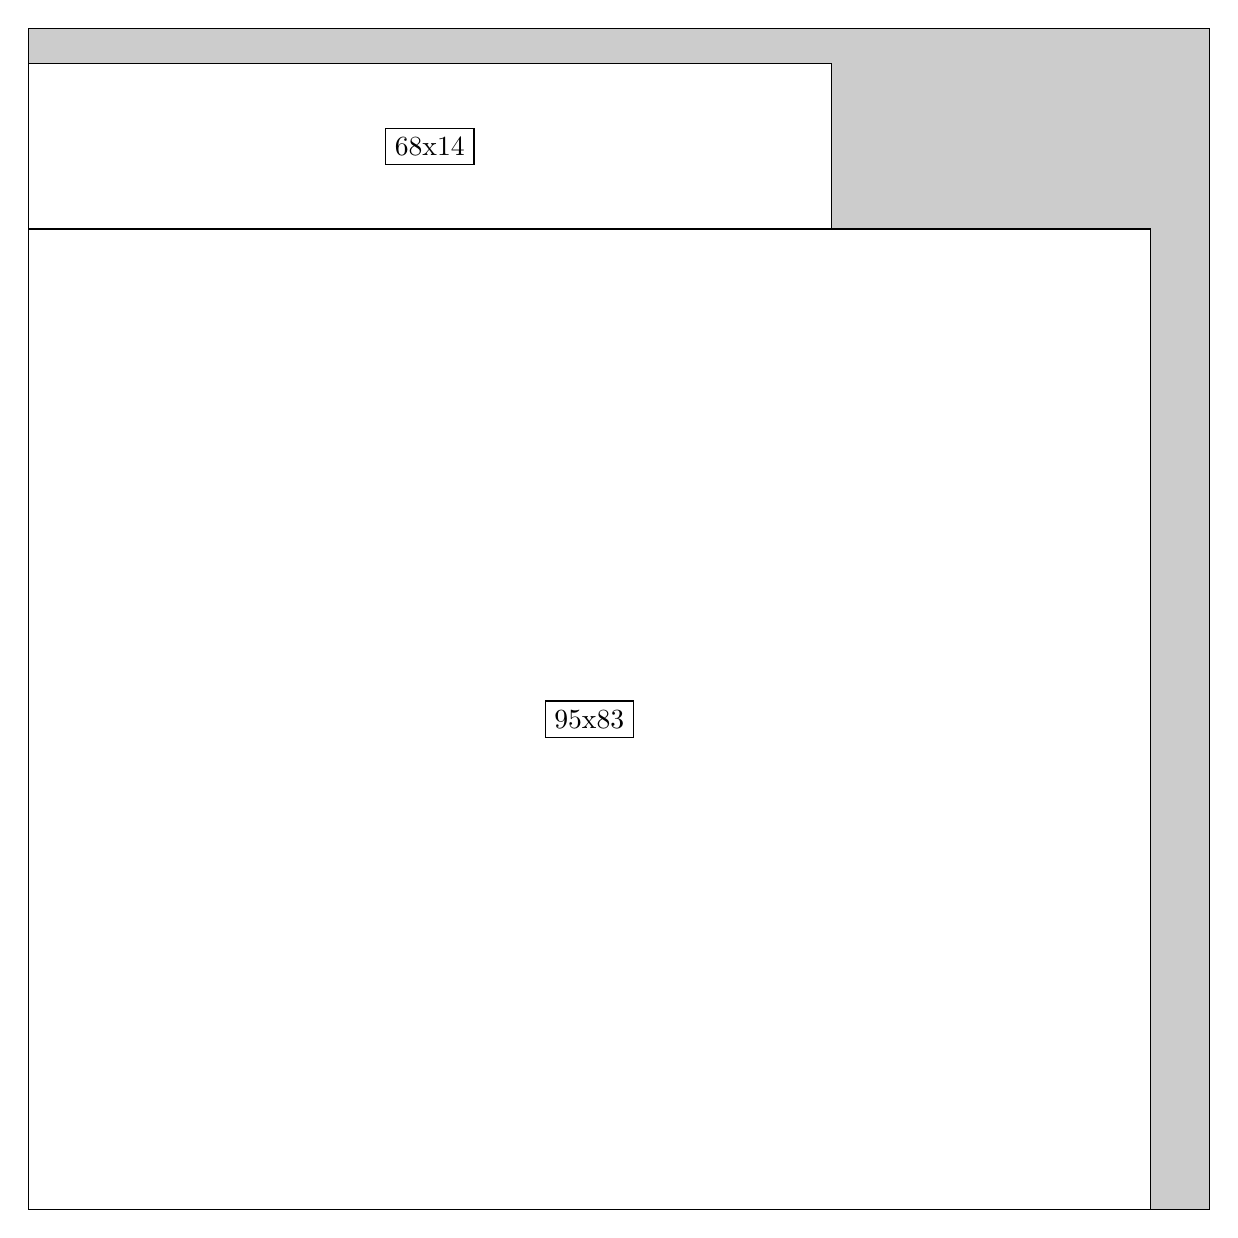
\begin{tikzpicture}[shorten >=1pt,scale=1.0,every node/.style={scale=1.0},->]
\tikzstyle{vertex}=[circle,fill=black!25,minimum size=14pt,inner sep=0pt]
\filldraw[fill=gray!40!white, draw=black] (0,0) rectangle (15.0,15.0);
\foreach \name/\x/\y/\w/\h in {95x83/0.0/0.0/14.25/12.45,68x14/0.0/12.45/10.2/2.1}
\filldraw[fill=white!40!white, draw=black] (\x,\y) rectangle node[draw] (\name) {\name} ++(\w,\h);
\end{tikzpicture}


w =95 , h =83 , x =0 , y =0 , v =7885
\par
w =68 , h =14 , x =0 , y =83 , v =952
\par
\newpage


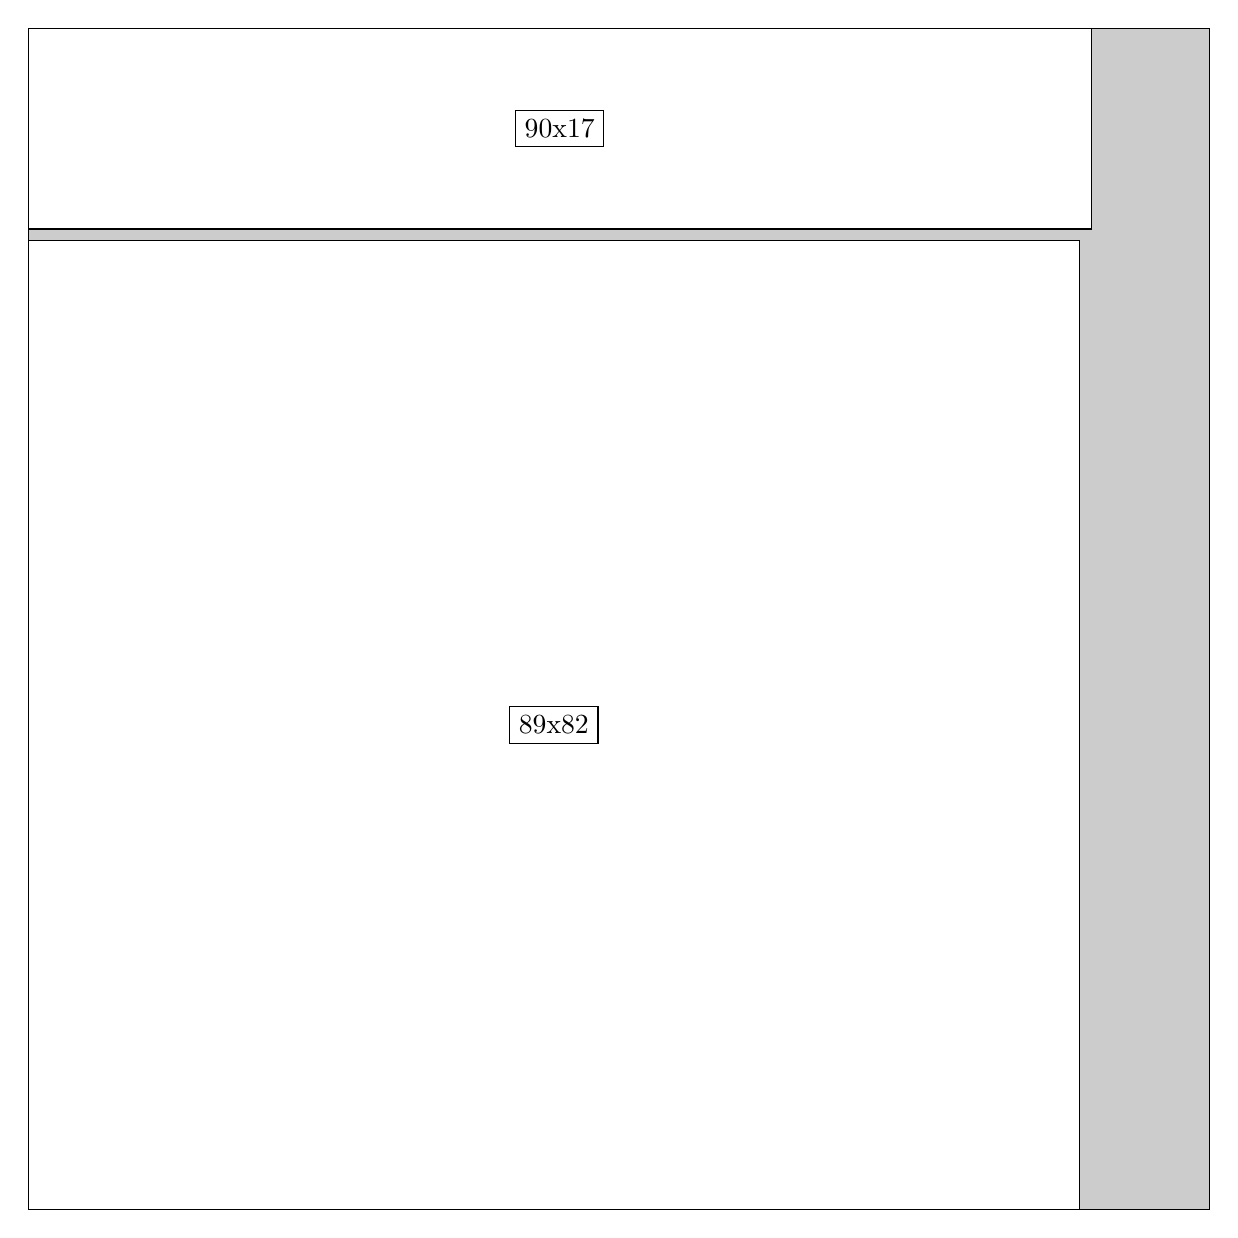
\begin{tikzpicture}[shorten >=1pt,scale=1.0,every node/.style={scale=1.0},->]
\tikzstyle{vertex}=[circle,fill=black!25,minimum size=14pt,inner sep=0pt]
\filldraw[fill=gray!40!white, draw=black] (0,0) rectangle (15.0,15.0);
\foreach \name/\x/\y/\w/\h in {89x82/0.0/0.0/13.35/12.299999999999999,90x17/0.0/12.45/13.5/2.55}
\filldraw[fill=white!40!white, draw=black] (\x,\y) rectangle node[draw] (\name) {\name} ++(\w,\h);
\end{tikzpicture}


w =89 , h =82 , x =0 , y =0 , v =7298
\par
w =90 , h =17 , x =0 , y =83 , v =1530
\par
\newpage


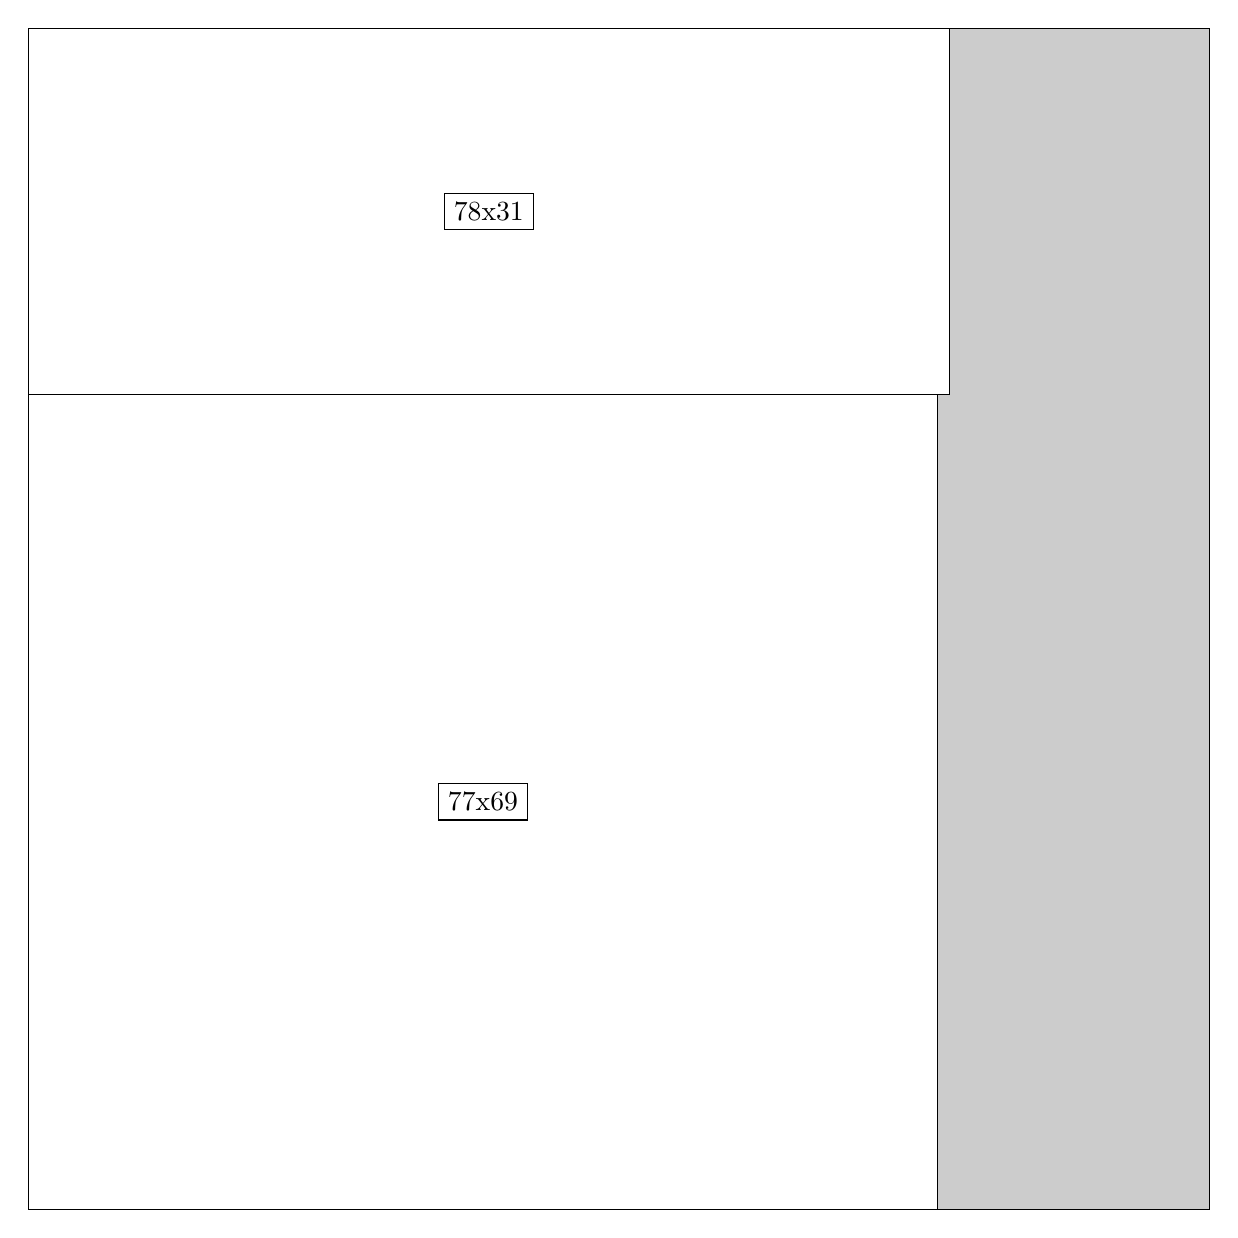
\begin{tikzpicture}[shorten >=1pt,scale=1.0,every node/.style={scale=1.0},->]
\tikzstyle{vertex}=[circle,fill=black!25,minimum size=14pt,inner sep=0pt]
\filldraw[fill=gray!40!white, draw=black] (0,0) rectangle (15.0,15.0);
\foreach \name/\x/\y/\w/\h in {77x69/0.0/0.0/11.549999999999999/10.35,78x31/0.0/10.35/11.7/4.6499999999999995}
\filldraw[fill=white!40!white, draw=black] (\x,\y) rectangle node[draw] (\name) {\name} ++(\w,\h);
\end{tikzpicture}


w =77 , h =69 , x =0 , y =0 , v =5313
\par
w =78 , h =31 , x =0 , y =69 , v =2418
\par
\newpage


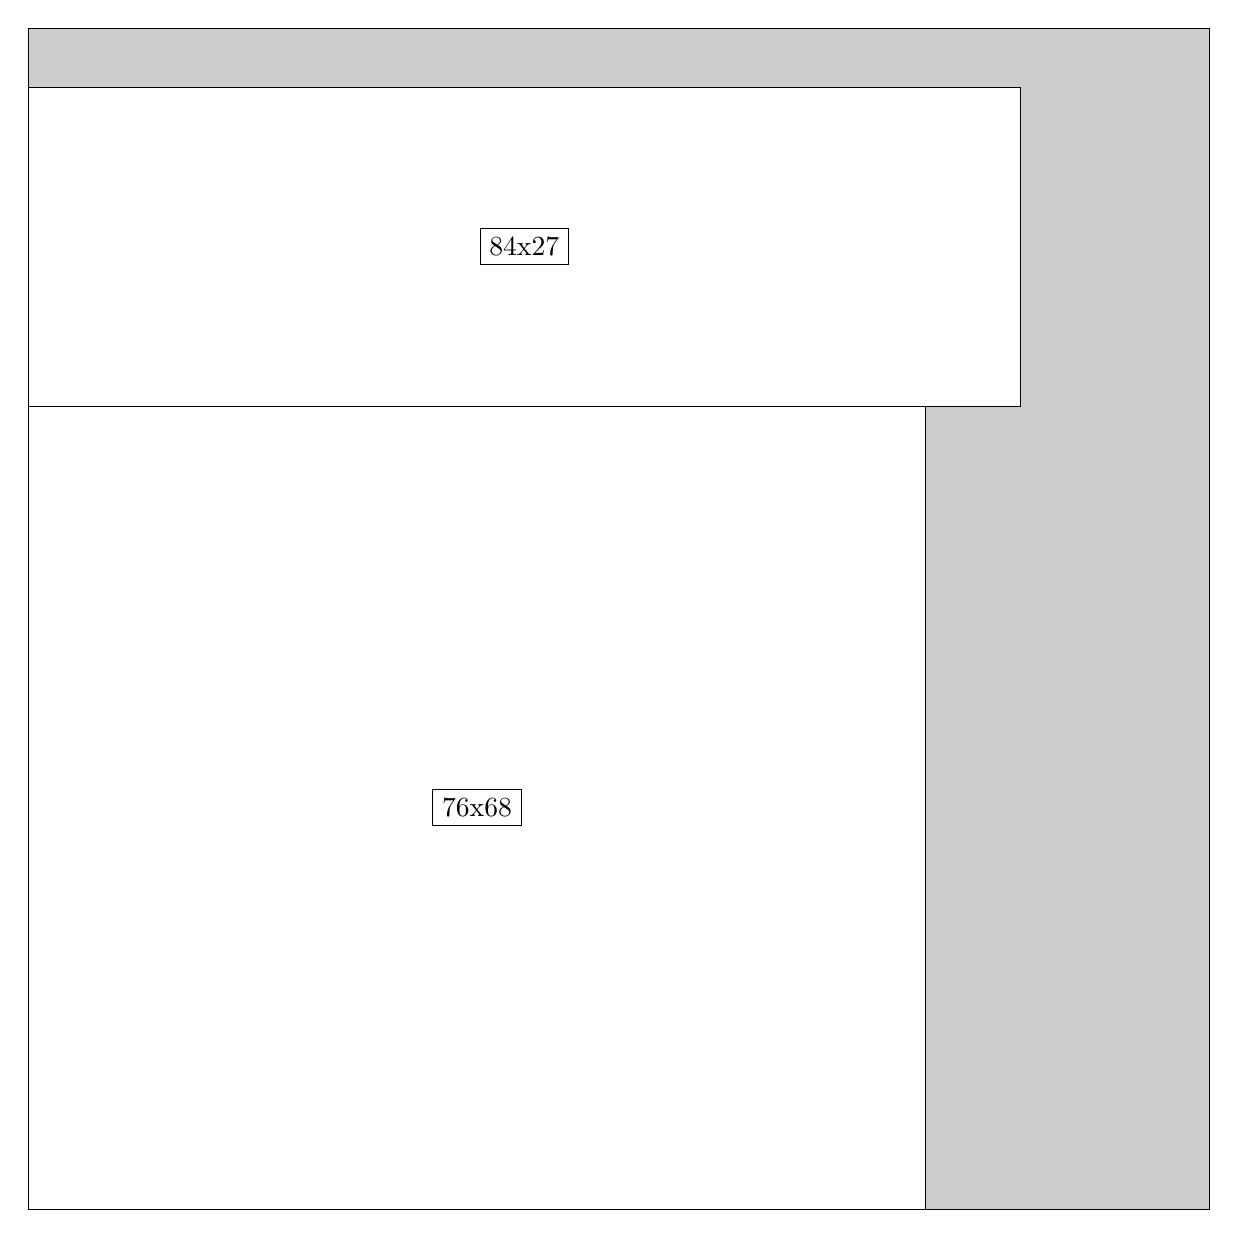
\begin{tikzpicture}[shorten >=1pt,scale=1.0,every node/.style={scale=1.0},->]
\tikzstyle{vertex}=[circle,fill=black!25,minimum size=14pt,inner sep=0pt]
\filldraw[fill=gray!40!white, draw=black] (0,0) rectangle (15.0,15.0);
\foreach \name/\x/\y/\w/\h in {76x68/0.0/0.0/11.4/10.2,84x27/0.0/10.2/12.6/4.05}
\filldraw[fill=white!40!white, draw=black] (\x,\y) rectangle node[draw] (\name) {\name} ++(\w,\h);
\end{tikzpicture}


w =76 , h =68 , x =0 , y =0 , v =5168
\par
w =84 , h =27 , x =0 , y =68 , v =2268
\par
\newpage


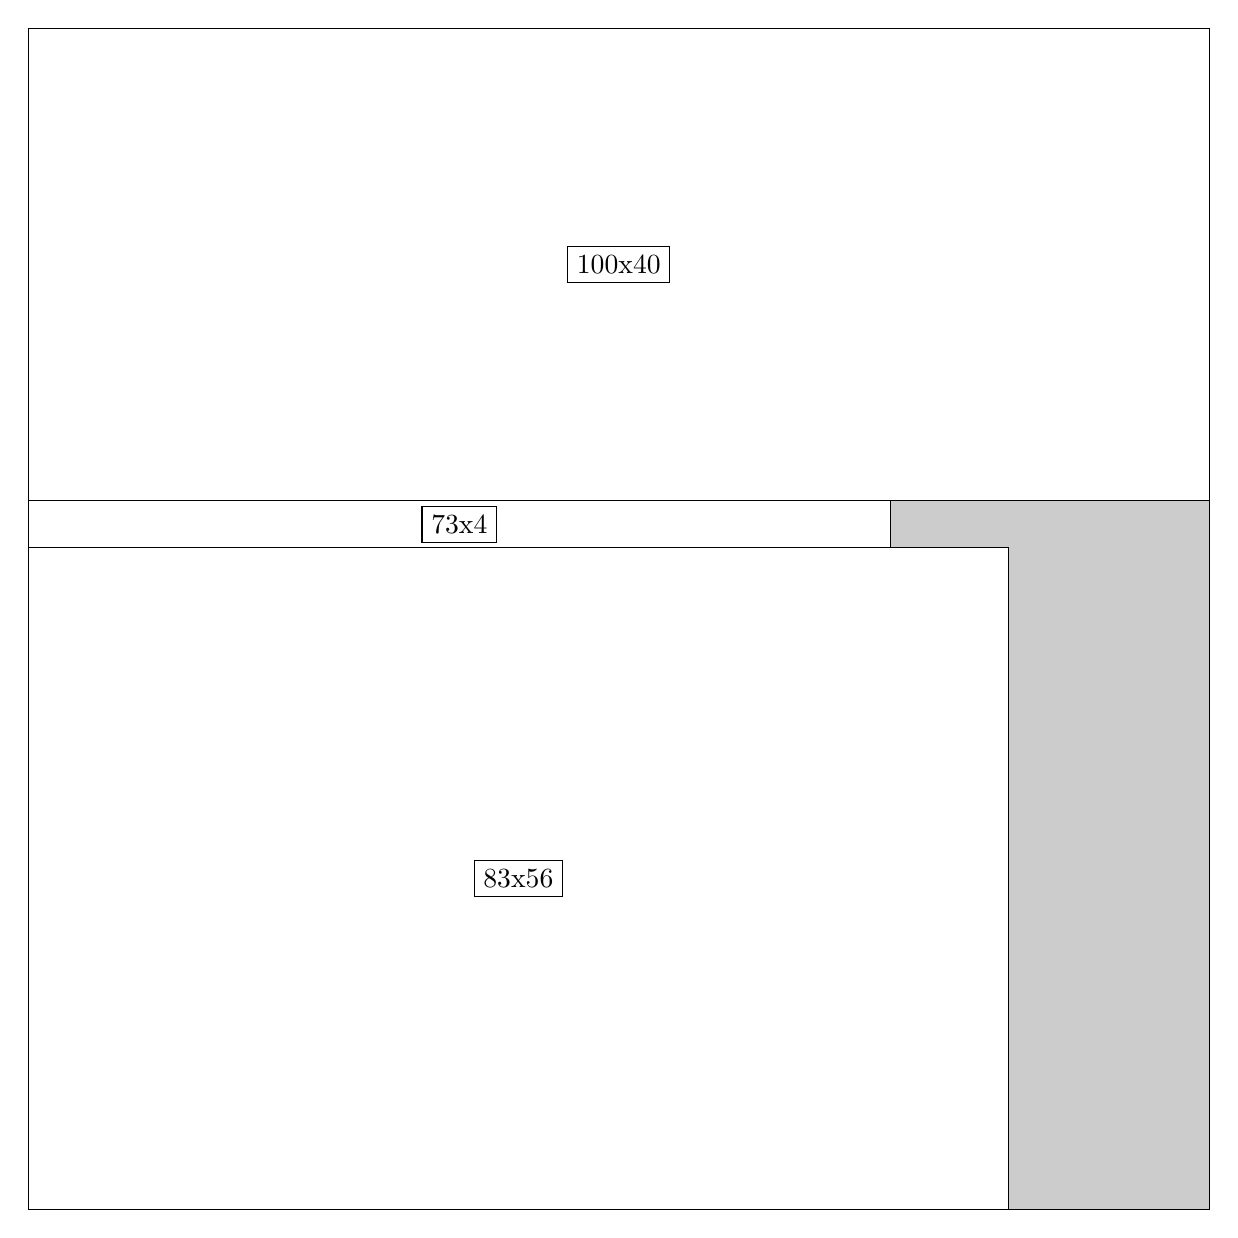
\begin{tikzpicture}[shorten >=1pt,scale=1.0,every node/.style={scale=1.0},->]
\tikzstyle{vertex}=[circle,fill=black!25,minimum size=14pt,inner sep=0pt]
\filldraw[fill=gray!40!white, draw=black] (0,0) rectangle (15.0,15.0);
\foreach \name/\x/\y/\w/\h in {83x56/0.0/0.0/12.45/8.4,100x40/0.0/9.0/15.0/6.0,73x4/0.0/8.4/10.95/0.6}
\filldraw[fill=white!40!white, draw=black] (\x,\y) rectangle node[draw] (\name) {\name} ++(\w,\h);
\end{tikzpicture}


w =83 , h =56 , x =0 , y =0 , v =4648
\par
w =100 , h =40 , x =0 , y =60 , v =4000
\par
w =73 , h =4 , x =0 , y =56 , v =292
\par
\newpage


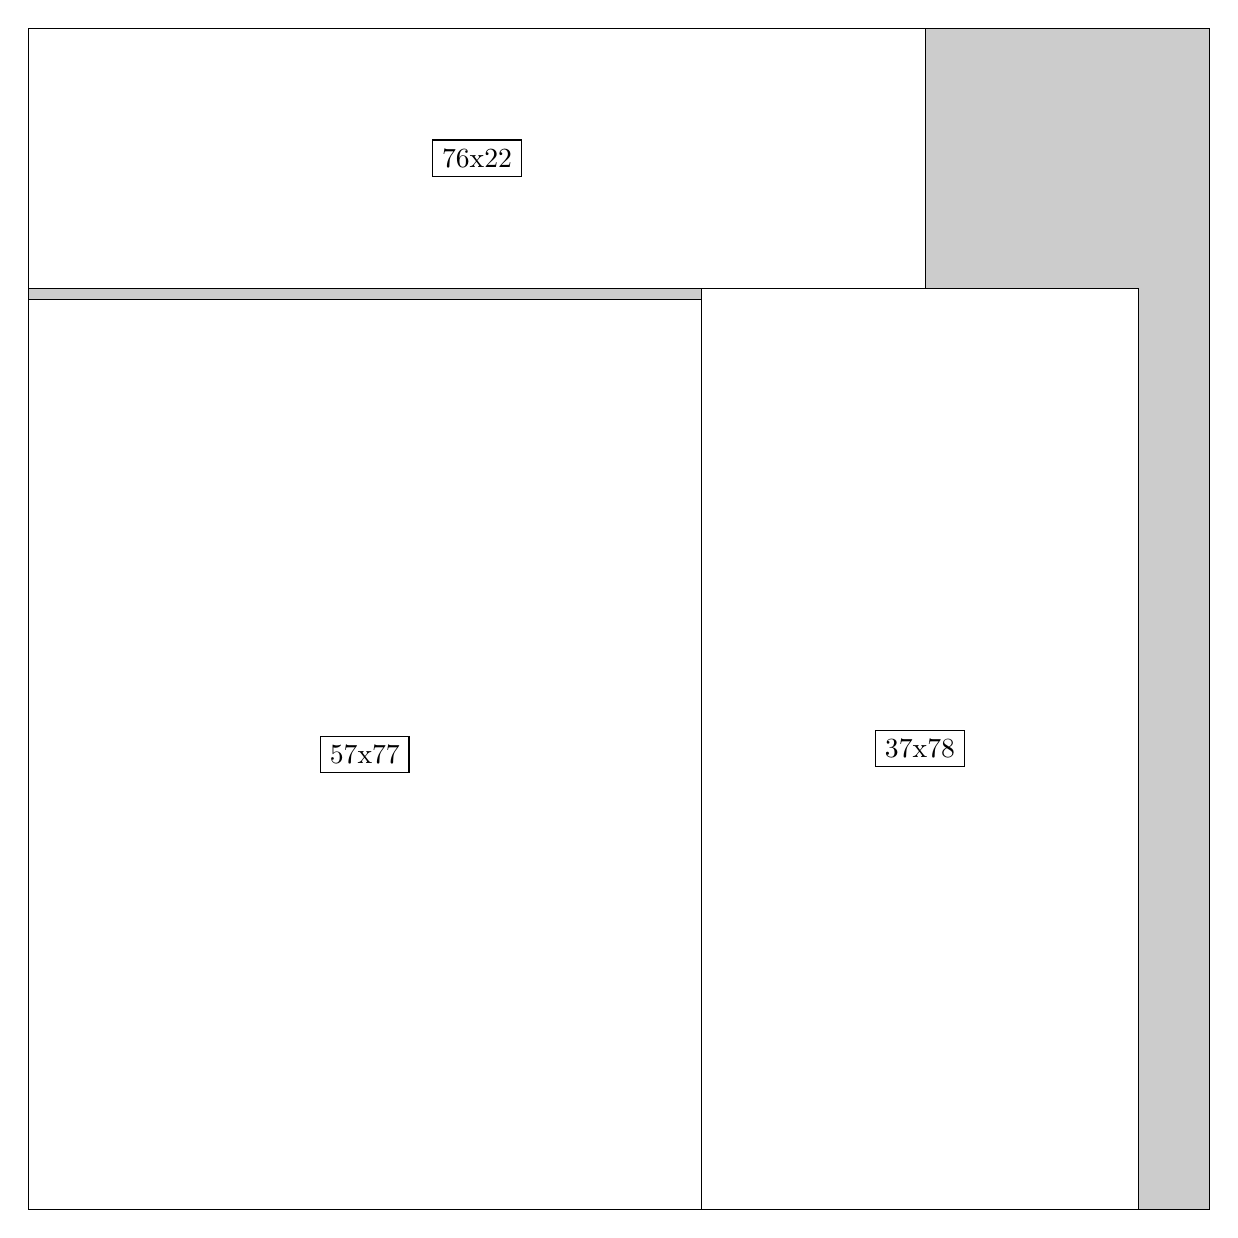
\begin{tikzpicture}[shorten >=1pt,scale=1.0,every node/.style={scale=1.0},->]
\tikzstyle{vertex}=[circle,fill=black!25,minimum size=14pt,inner sep=0pt]
\filldraw[fill=gray!40!white, draw=black] (0,0) rectangle (15.0,15.0);
\foreach \name/\x/\y/\w/\h in {57x77/0.0/0.0/8.549999999999999/11.549999999999999,37x78/8.549999999999999/0.0/5.55/11.7,76x22/0.0/11.7/11.4/3.3}
\filldraw[fill=white!40!white, draw=black] (\x,\y) rectangle node[draw] (\name) {\name} ++(\w,\h);
\end{tikzpicture}


w =57 , h =77 , x =0 , y =0 , v =4389
\par
w =37 , h =78 , x =57 , y =0 , v =2886
\par
w =76 , h =22 , x =0 , y =78 , v =1672
\par
\newpage


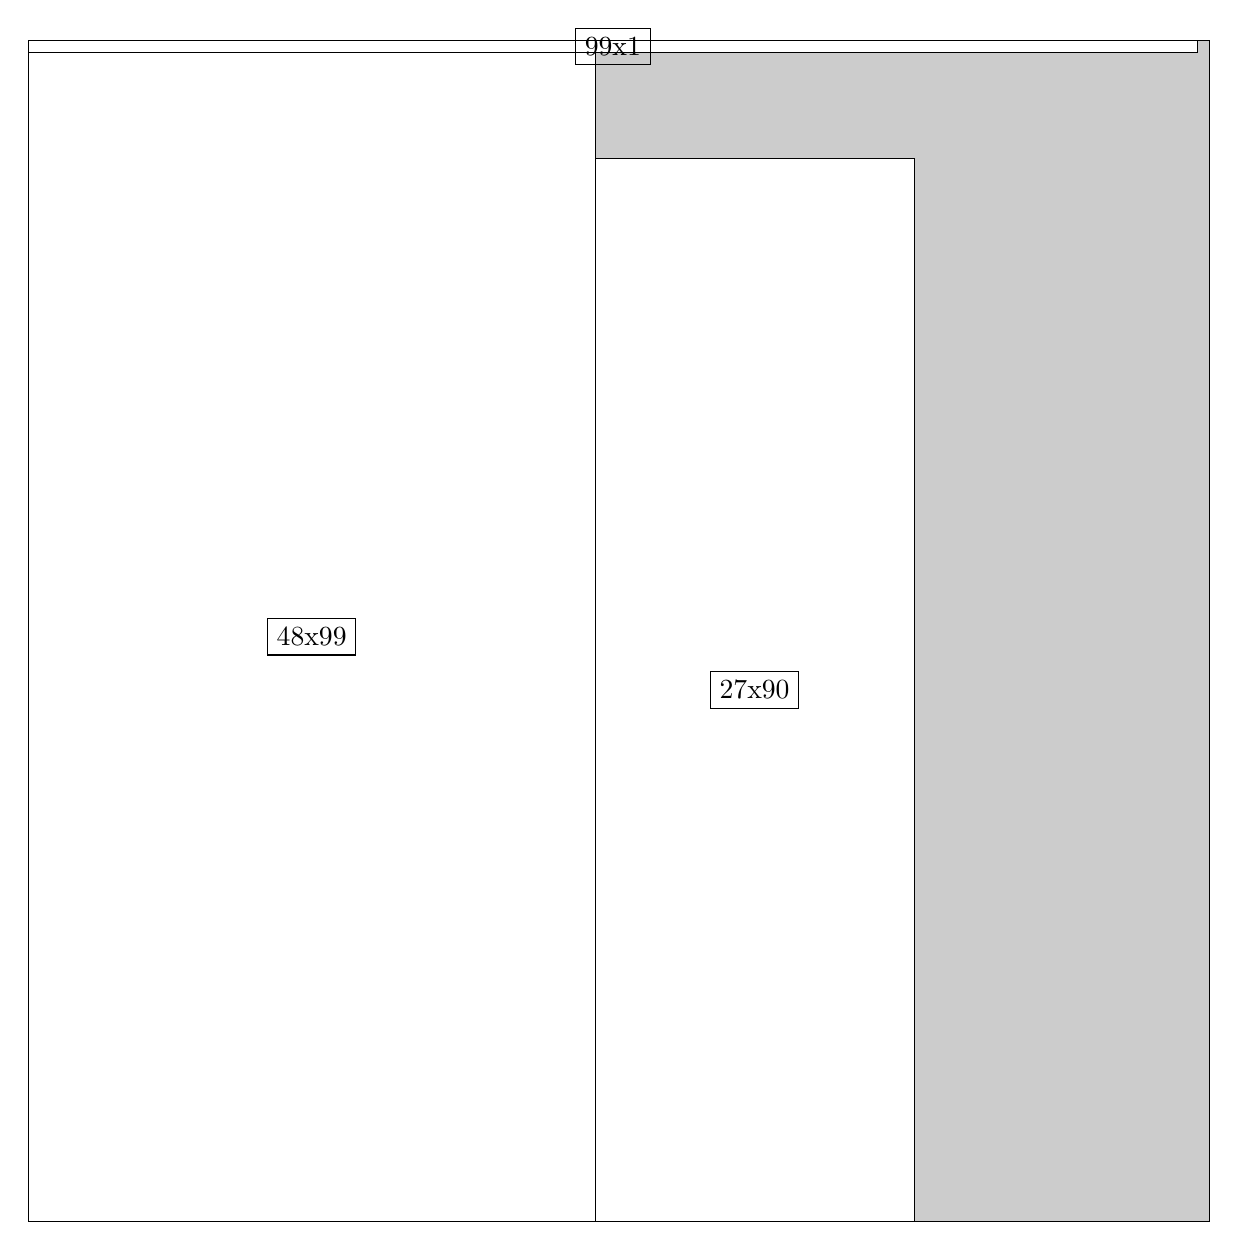
\begin{tikzpicture}[shorten >=1pt,scale=1.0,every node/.style={scale=1.0},->]
\tikzstyle{vertex}=[circle,fill=black!25,minimum size=14pt,inner sep=0pt]
\filldraw[fill=gray!40!white, draw=black] (0,0) rectangle (15.0,15.0);
\foreach \name/\x/\y/\w/\h in {48x99/0.0/0.0/7.199999999999999/14.85,27x90/7.199999999999999/0.0/4.05/13.5,99x1/0.0/14.85/14.85/0.15}
\filldraw[fill=white!40!white, draw=black] (\x,\y) rectangle node[draw] (\name) {\name} ++(\w,\h);
\end{tikzpicture}


w =48 , h =99 , x =0 , y =0 , v =4752
\par
w =27 , h =90 , x =48 , y =0 , v =2430
\par
w =99 , h =1 , x =0 , y =99 , v =99
\par
\newpage


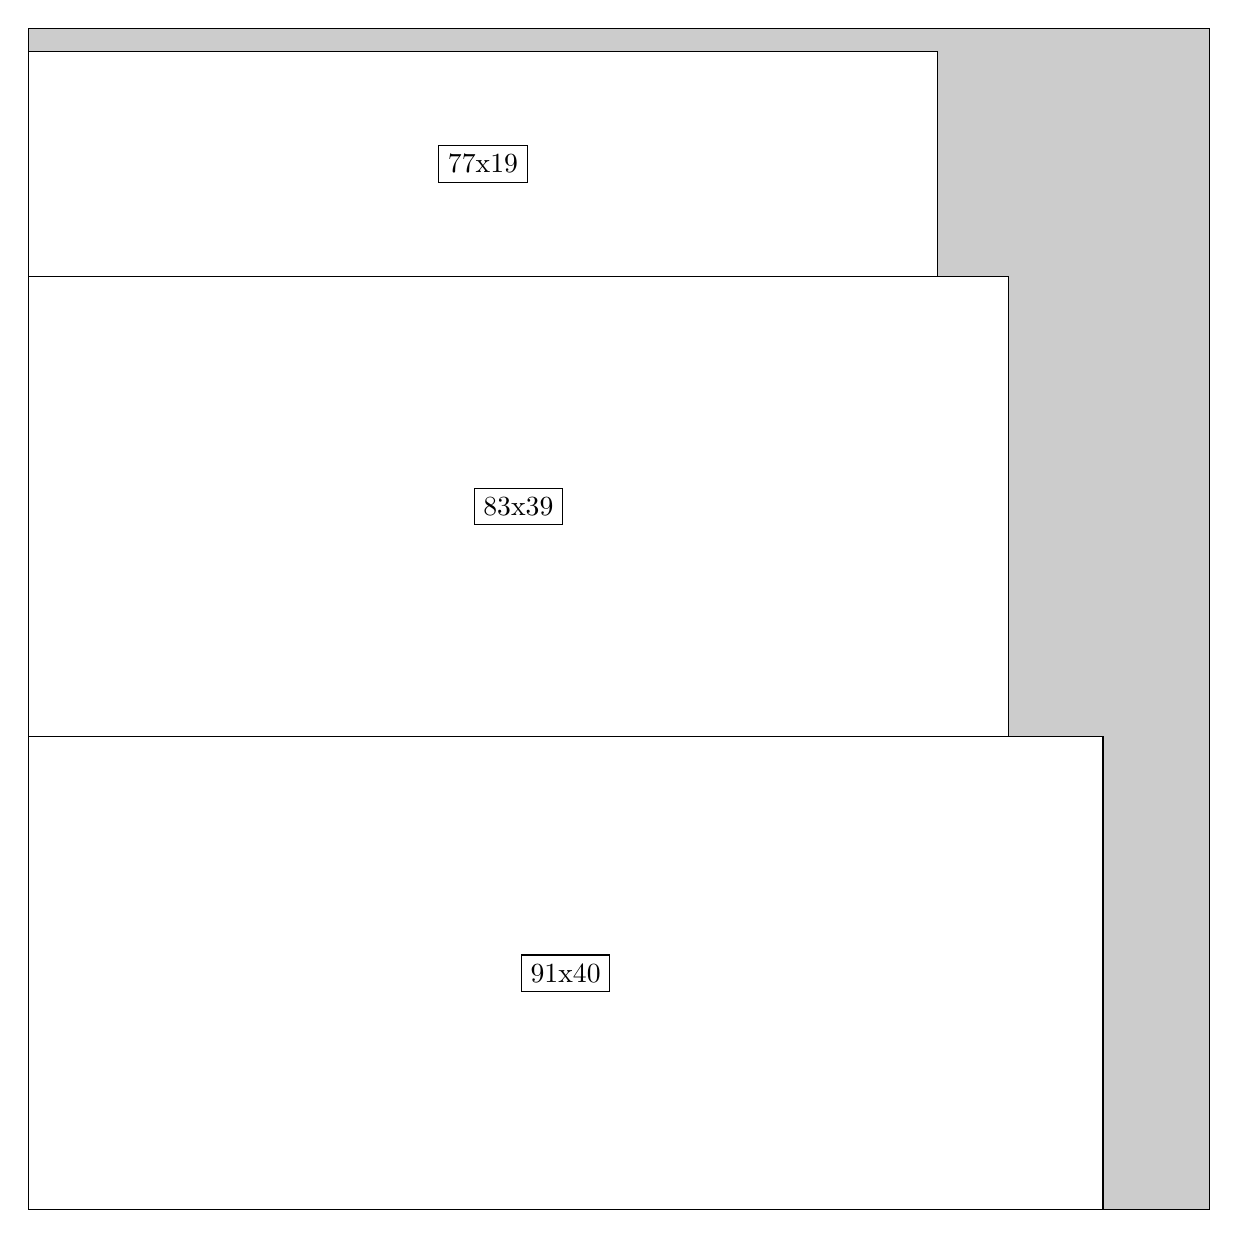
\begin{tikzpicture}[shorten >=1pt,scale=1.0,every node/.style={scale=1.0},->]
\tikzstyle{vertex}=[circle,fill=black!25,minimum size=14pt,inner sep=0pt]
\filldraw[fill=gray!40!white, draw=black] (0,0) rectangle (15.0,15.0);
\foreach \name/\x/\y/\w/\h in {91x40/0.0/0.0/13.65/6.0,83x39/0.0/6.0/12.45/5.85,77x19/0.0/11.85/11.549999999999999/2.85}
\filldraw[fill=white!40!white, draw=black] (\x,\y) rectangle node[draw] (\name) {\name} ++(\w,\h);
\end{tikzpicture}


w =91 , h =40 , x =0 , y =0 , v =3640
\par
w =83 , h =39 , x =0 , y =40 , v =3237
\par
w =77 , h =19 , x =0 , y =79 , v =1463
\par
\newpage


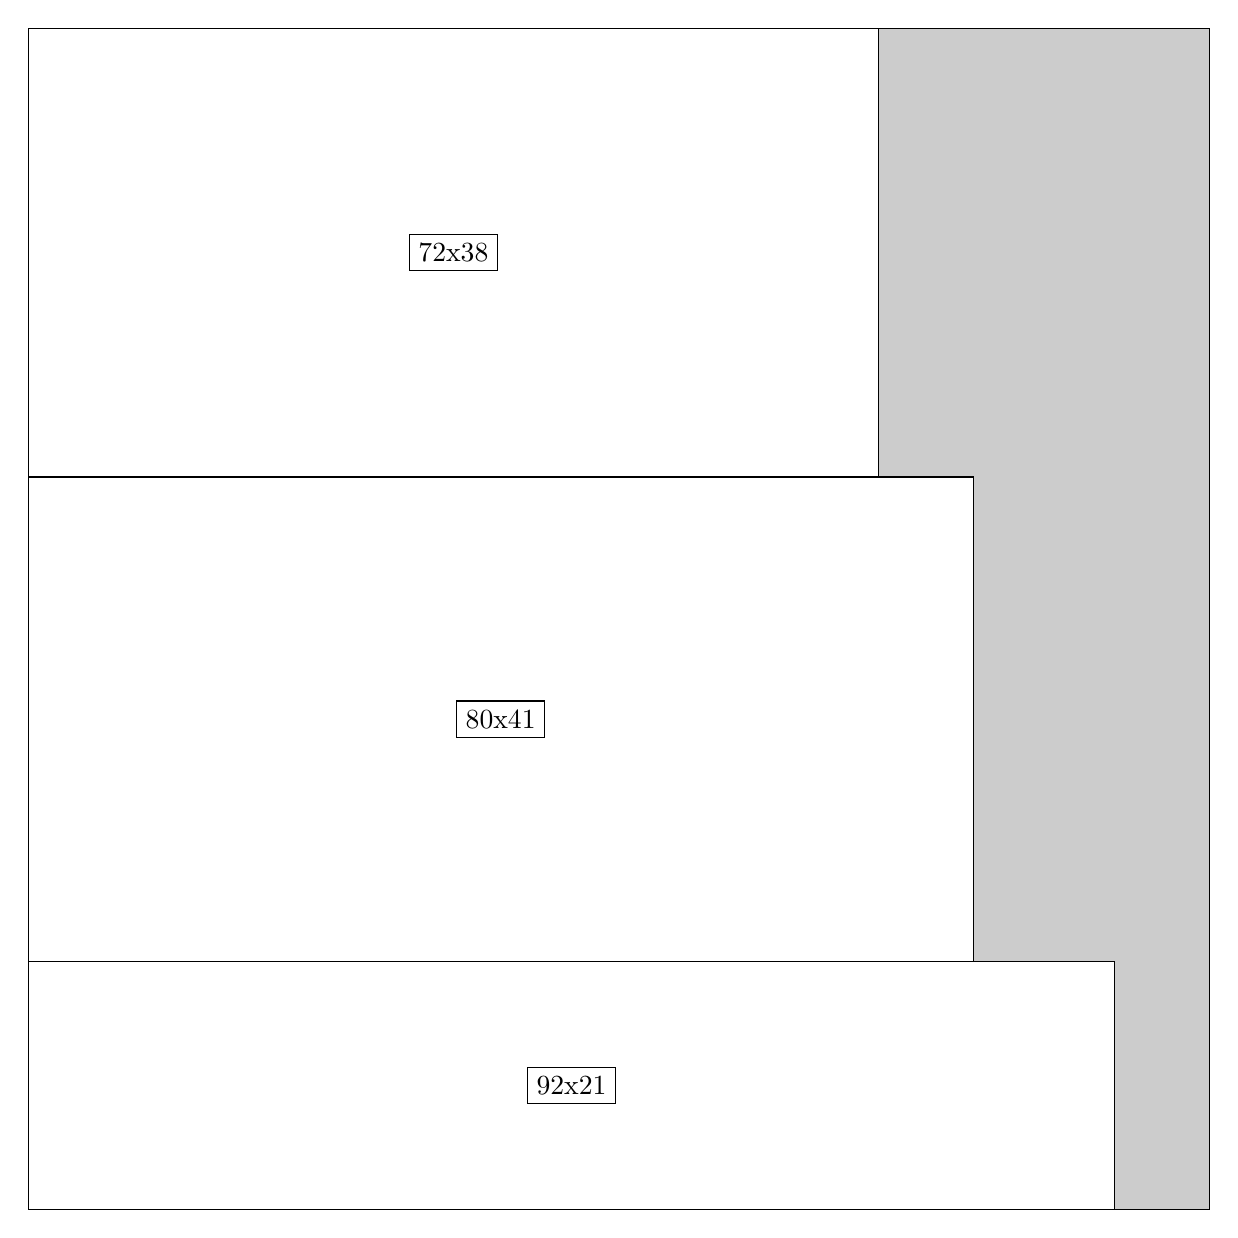
\begin{tikzpicture}[shorten >=1pt,scale=1.0,every node/.style={scale=1.0},->]
\tikzstyle{vertex}=[circle,fill=black!25,minimum size=14pt,inner sep=0pt]
\filldraw[fill=gray!40!white, draw=black] (0,0) rectangle (15.0,15.0);
\foreach \name/\x/\y/\w/\h in {80x41/0.0/3.15/12.0/6.1499999999999995,72x38/0.0/9.299999999999999/10.799999999999999/5.7,92x21/0.0/0.0/13.799999999999999/3.15}
\filldraw[fill=white!40!white, draw=black] (\x,\y) rectangle node[draw] (\name) {\name} ++(\w,\h);
\end{tikzpicture}


w =80 , h =41 , x =0 , y =21 , v =3280
\par
w =72 , h =38 , x =0 , y =62 , v =2736
\par
w =92 , h =21 , x =0 , y =0 , v =1932
\par
\newpage


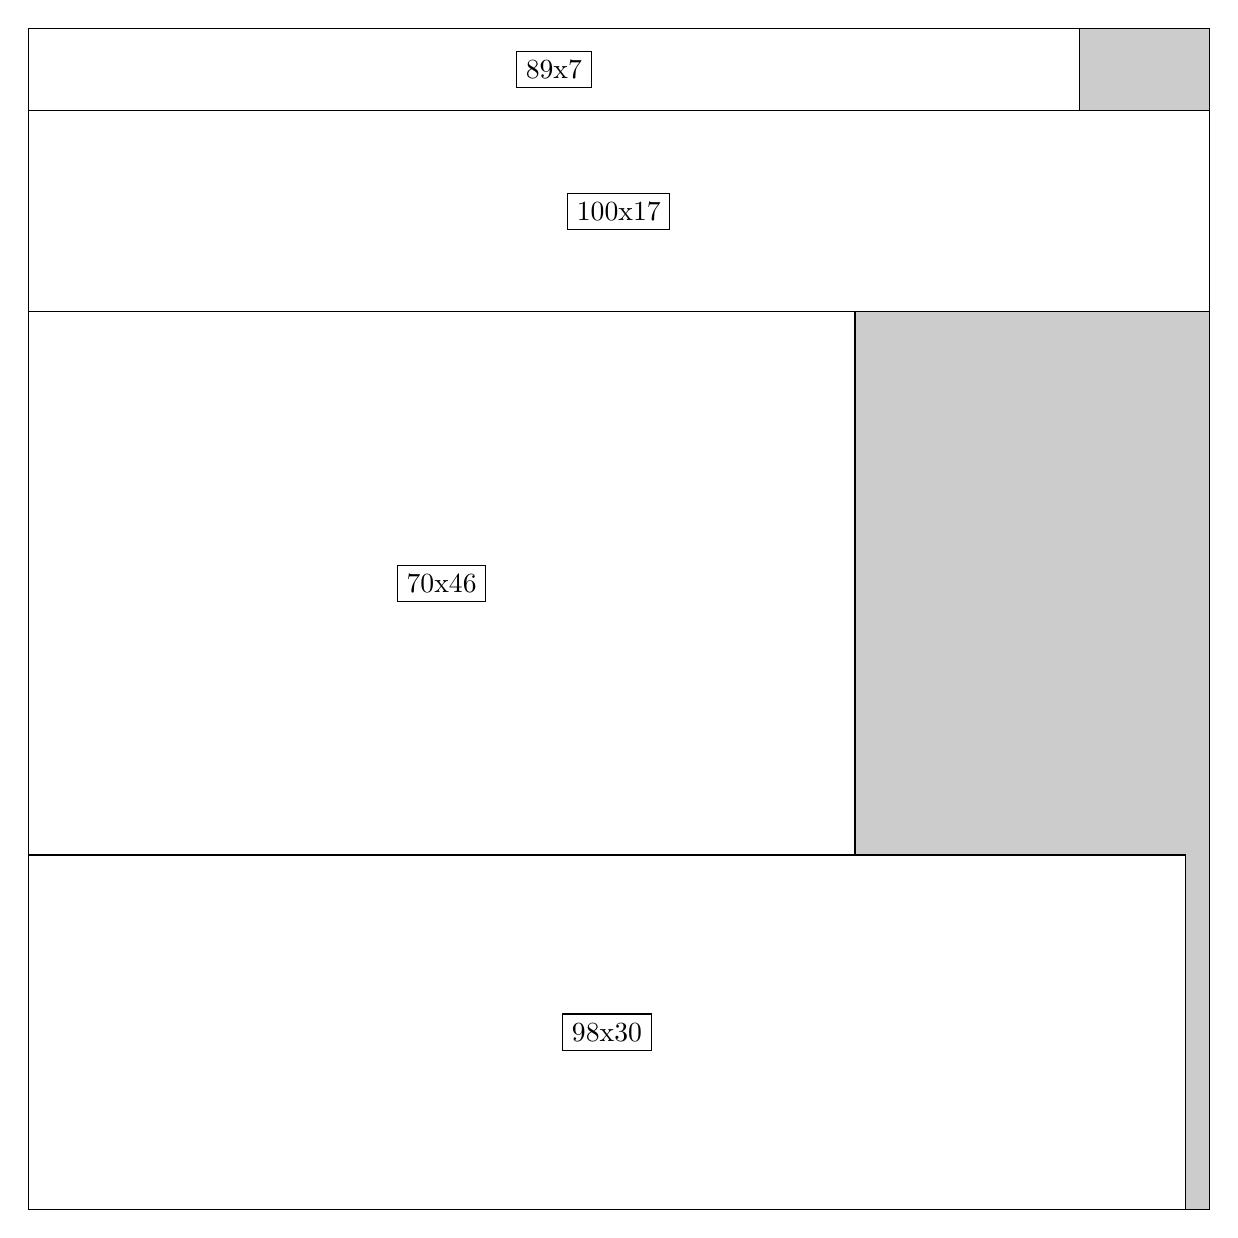
\begin{tikzpicture}[shorten >=1pt,scale=1.0,every node/.style={scale=1.0},->]
\tikzstyle{vertex}=[circle,fill=black!25,minimum size=14pt,inner sep=0pt]
\filldraw[fill=gray!40!white, draw=black] (0,0) rectangle (15.0,15.0);
\foreach \name/\x/\y/\w/\h in {70x46/0.0/4.5/10.5/6.8999999999999995,100x17/0.0/11.4/15.0/2.55,98x30/0.0/0.0/14.7/4.5,89x7/0.0/13.95/13.35/1.05}
\filldraw[fill=white!40!white, draw=black] (\x,\y) rectangle node[draw] (\name) {\name} ++(\w,\h);
\end{tikzpicture}


w =70 , h =46 , x =0 , y =30 , v =3220
\par
w =100 , h =17 , x =0 , y =76 , v =1700
\par
w =98 , h =30 , x =0 , y =0 , v =2940
\par
w =89 , h =7 , x =0 , y =93 , v =623
\par
\newpage


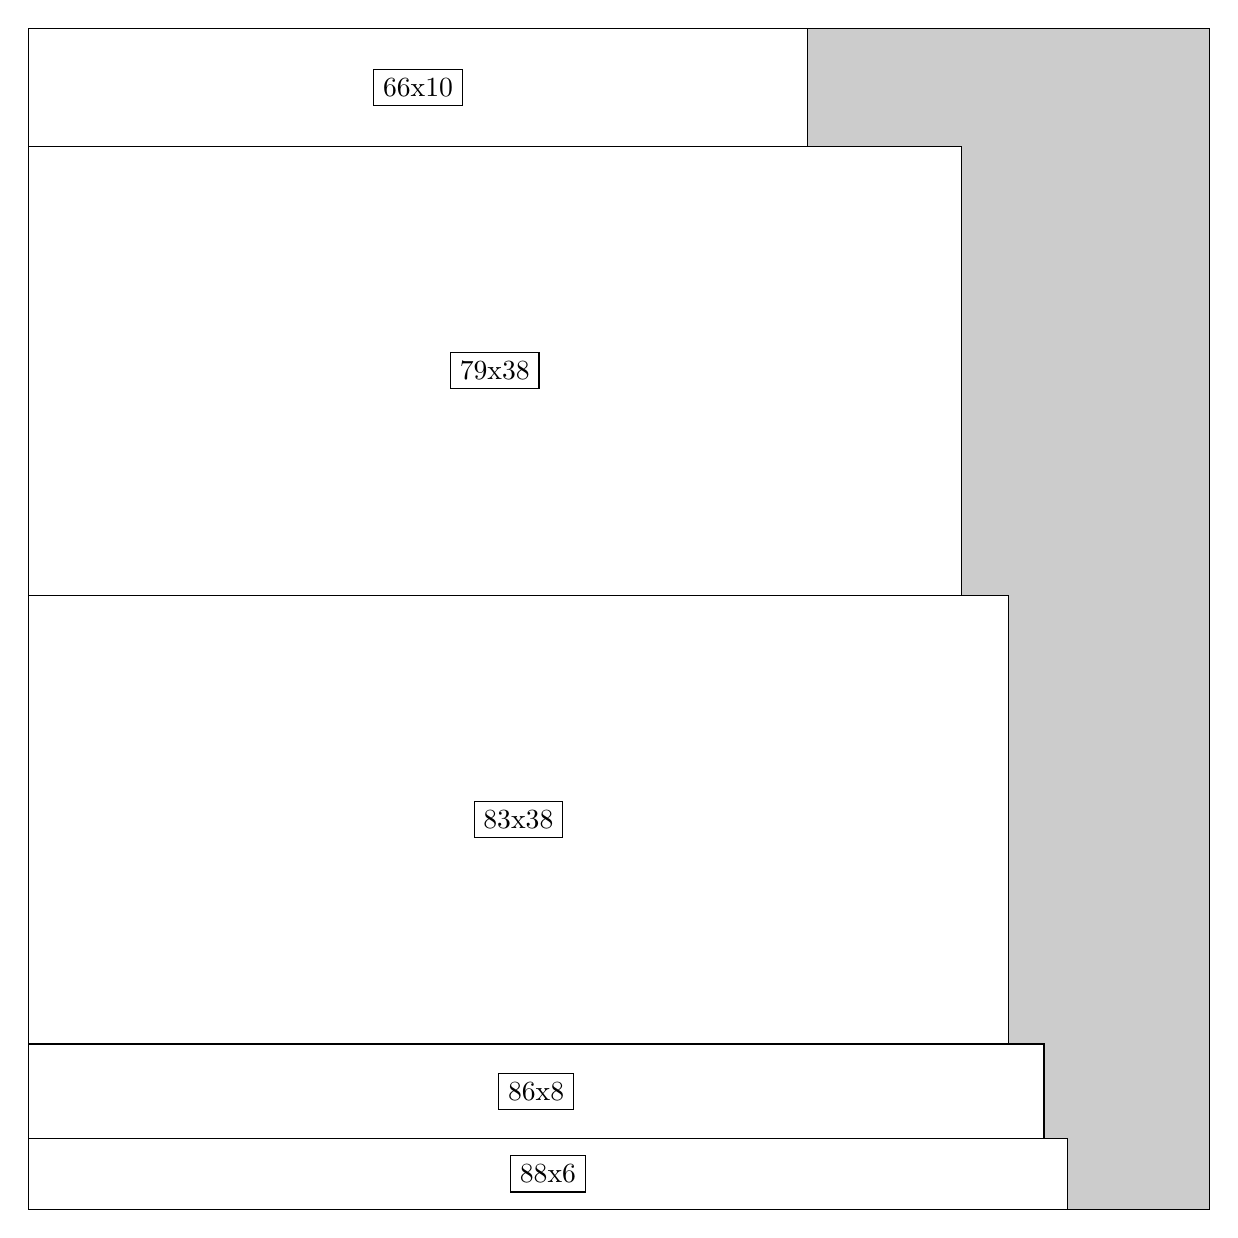
\begin{tikzpicture}[shorten >=1pt,scale=1.0,every node/.style={scale=1.0},->]
\tikzstyle{vertex}=[circle,fill=black!25,minimum size=14pt,inner sep=0pt]
\filldraw[fill=gray!40!white, draw=black] (0,0) rectangle (15.0,15.0);
\foreach \name/\x/\y/\w/\h in {83x38/0.0/2.1/12.45/5.7,79x38/0.0/7.8/11.85/5.7,86x8/0.0/0.8999999999999999/12.9/1.2,66x10/0.0/13.5/9.9/1.5,88x6/0.0/0.0/13.2/0.8999999999999999}
\filldraw[fill=white!40!white, draw=black] (\x,\y) rectangle node[draw] (\name) {\name} ++(\w,\h);
\end{tikzpicture}


w =83 , h =38 , x =0 , y =14 , v =3154
\par
w =79 , h =38 , x =0 , y =52 , v =3002
\par
w =86 , h =8 , x =0 , y =6 , v =688
\par
w =66 , h =10 , x =0 , y =90 , v =660
\par
w =88 , h =6 , x =0 , y =0 , v =528
\par
\newpage


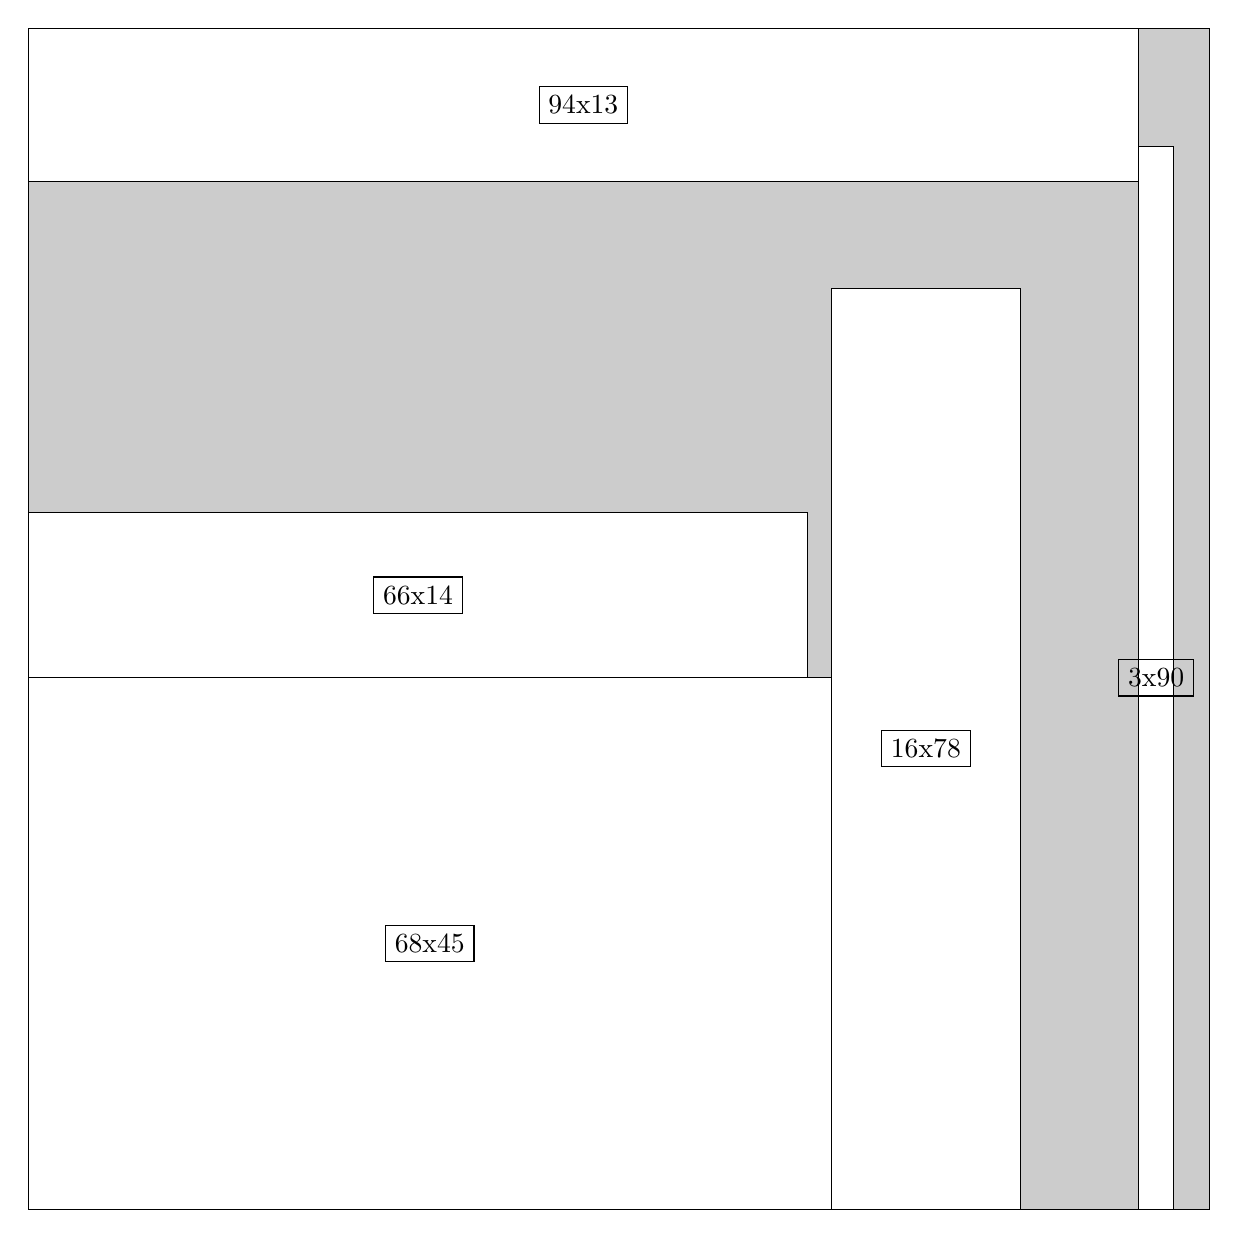
\begin{tikzpicture}[shorten >=1pt,scale=1.0,every node/.style={scale=1.0},->]
\tikzstyle{vertex}=[circle,fill=black!25,minimum size=14pt,inner sep=0pt]
\filldraw[fill=gray!40!white, draw=black] (0,0) rectangle (15.0,15.0);
\foreach \name/\x/\y/\w/\h in {68x45/0.0/0.0/10.2/6.75,16x78/10.2/0.0/2.4/11.7,3x90/14.1/0.0/0.44999999999999996/13.5,66x14/0.0/6.75/9.9/2.1,94x13/0.0/13.049999999999999/14.1/1.95}
\filldraw[fill=white!40!white, draw=black] (\x,\y) rectangle node[draw] (\name) {\name} ++(\w,\h);
\end{tikzpicture}


w =68 , h =45 , x =0 , y =0 , v =3060
\par
w =16 , h =78 , x =68 , y =0 , v =1248
\par
w =3 , h =90 , x =94 , y =0 , v =270
\par
w =66 , h =14 , x =0 , y =45 , v =924
\par
w =94 , h =13 , x =0 , y =87 , v =1222
\par
\newpage


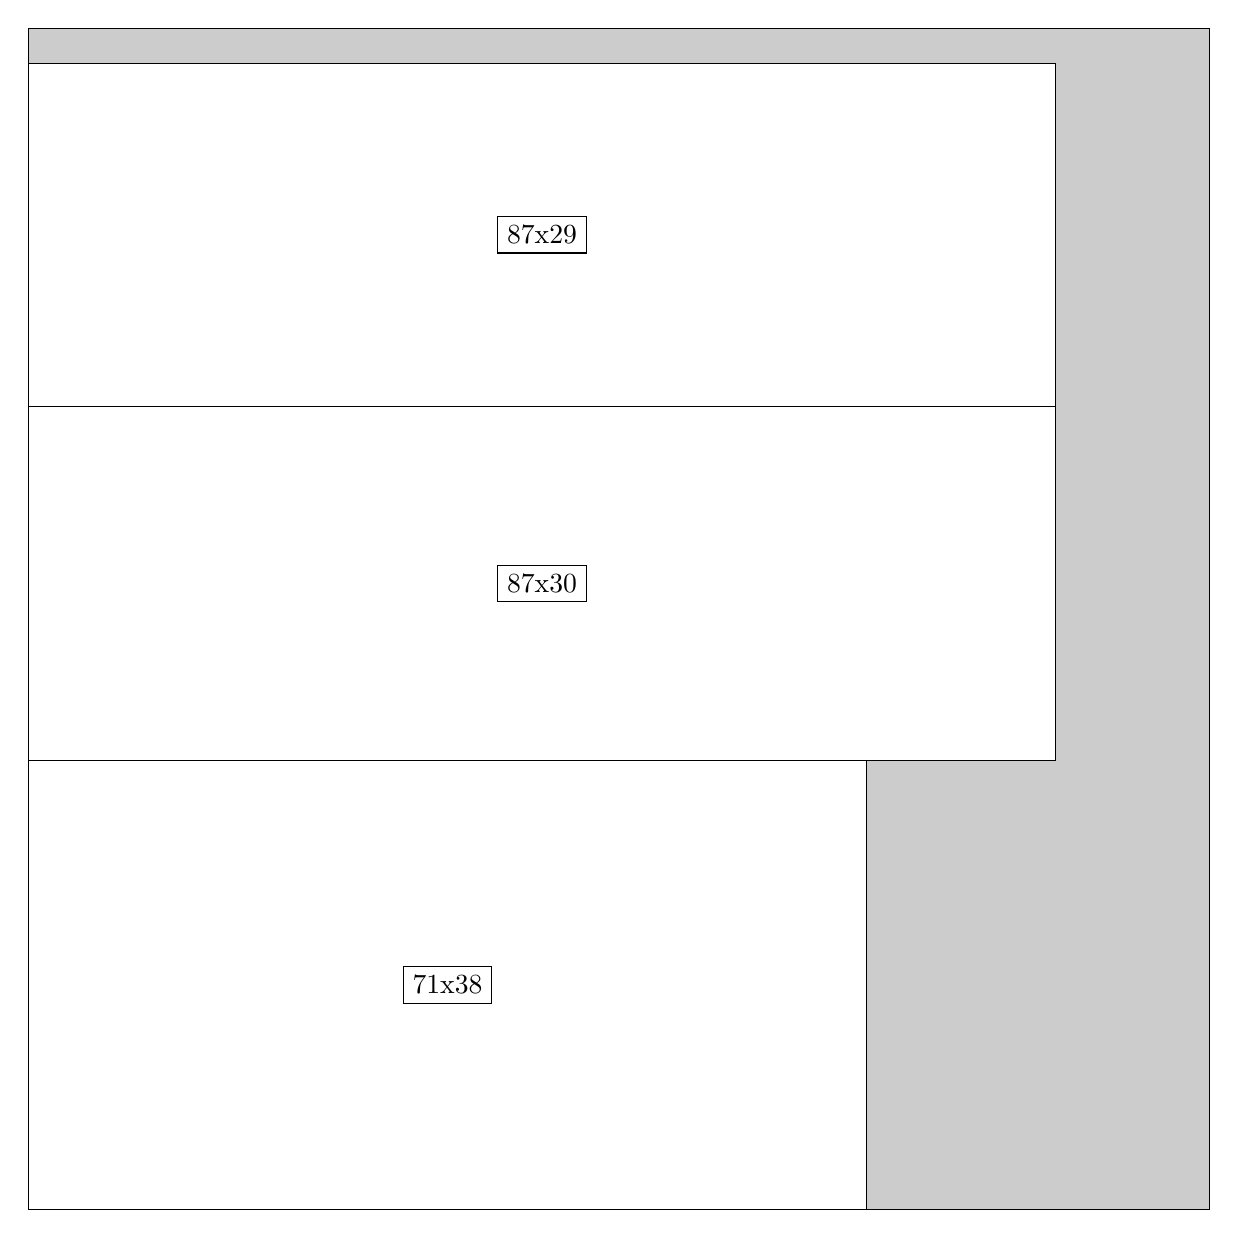
\begin{tikzpicture}[shorten >=1pt,scale=1.0,every node/.style={scale=1.0},->]
\tikzstyle{vertex}=[circle,fill=black!25,minimum size=14pt,inner sep=0pt]
\filldraw[fill=gray!40!white, draw=black] (0,0) rectangle (15.0,15.0);
\foreach \name/\x/\y/\w/\h in {71x38/0.0/0.0/10.65/5.7,87x30/0.0/5.7/13.049999999999999/4.5,87x29/0.0/10.2/13.049999999999999/4.35}
\filldraw[fill=white!40!white, draw=black] (\x,\y) rectangle node[draw] (\name) {\name} ++(\w,\h);
\end{tikzpicture}


w =71 , h =38 , x =0 , y =0 , v =2698
\par
w =87 , h =30 , x =0 , y =38 , v =2610
\par
w =87 , h =29 , x =0 , y =68 , v =2523
\par
\newpage


\end{document}